%% Generated by docs/paper/render_latex.py --mode journal — do not edit by hand.
%% Edit the prose in docs/paper/content.py, or re-run the experiment whose
%% artifact produced the number you want to change.
\documentclass[journal]{IEEEtran}

\usepackage{cite}
\usepackage{amsmath,amssymb}
\usepackage{graphicx}
\usepackage{booktabs}
\usepackage{multirow}
\usepackage{url}
\usepackage[hidelinks]{hyperref}
\usepackage{listings}
\usepackage{xcolor}

\lstset{
  basicstyle=\ttfamily\scriptsize,
  breaklines=true,
  frame=single,
  rulecolor=\color{black!30},
  columns=fullflexible,
  keepspaces=true,
}

\graphicspath{{figures/}}

\begin{document}

\title{Scale-Invariant Baselines Can Certify a Broken Deep Model: Grouped-Normalisation Collapse in Learned Trajectory Screening}

\author{
Harsha Vardan M Sakamuri, Rohit Michael, Valarmathi Sudhakar
\thanks{All authors are with the OrbitGuard Research Group.}
}

\maketitle


\begin{abstract}
Fitting one feature scaler across several groups of data is an ordinary thing to do. We show it can quietly destroy a sequence model while every check a practitioner would normally run says the pipeline is fine. On 70,000 simulated interplanetary trajectories across seven targets, a Transformer trained under a scaler pooled across a group of targets stops responding to its input on Venus: the standard deviation of its held-out prediction is 3.11e-05 and its validation AUC is 0.6037, against 0.9999 for the same architecture under per-timestep normalisation. Every one of the 1,500 held-out missions falls inside a window 3.2e-04 wide. A gradient-boosted tree fitted to the very same arrays does not notice: its AUC moves by at most 0.0002 across all three normalisation settings, and it reports the task as almost perfectly separable while the network cannot separate it at all. So the usual instinct (check a simple baseline before blaming the data) fails exactly here, because trees are invariant to the thing that breaks the network. The effect is severe but not universal: 1 of 4 targets collapses outright and the rest lose between 0.0003 and 0.0925 AUC while still working, so we report when it happens and when it does not. We separate the two kinds of pooling that are usually confused (pooling across timesteps is survivable, pooling across groups is not), give a diagnostic based on the spread of the predictions rather than on accuracy, and report a second failure of the same model, which cannot reach a rare class that a tree recovers from the identical input. Across 5 seeds the compression is identical and the collapse recurs on 4 of them, so it is a property of the preprocessing rather than of one unlucky initialisation.
\end{abstract}

\begin{IEEEkeywords}
feature normalisation, shortcut learning, model diagnostics, simulation screening, trajectory analysis, negative results
\end{IEEEkeywords}

\section{Introduction}

Monte Carlo trajectory campaigns spend most of their compute on runs that were already doomed when the spacecraft left its parking orbit. Flight projects run these campaigns as a matter of course; TESS, for one, used a large dispersion campaign to drive its trajectory design \cite{nickel2016montecarlo}. The cost is real enough that a body of work exists purely to make each propagation cheaper \cite{massari2017nonlinear,jia2022datadriven}. A different and obvious idea is to skip the runs instead: watch the first part of a trajectory and cancel the ones that are going to fail.

We built that screen. Doing so turned up two failures that we think matter well beyond astrodynamics, and one negative result about the screen itself.

The first failure is what this paper is about. A model trained on grouped data, with a single feature scaler fitted across the whole group, ended up emitting one constant number per group. What makes it worth writing down is not that it happened, but that it went unnoticed for a long time. Validation AUC stayed high, because a mixed validation set lets a model score well by telling groups apart without telling anything apart inside a group. A gradient-boosted baseline run on the same arrays reported near-perfect performance, because trees split on absolute values and simply do not care about the scaling the network depends on. Both of the checks we would have trusted said the pipeline was healthy.

This is uncomfortable, because running a simple baseline is good advice. Tree ensembles are the standard sanity check on tabular and physical data, and they are usually the right one \cite{chen2016xgboost,grinsztajn2022tree,shwartz2022tabular}. The problem is that the property that makes them a good check in general (invariance to how the features are scaled) is precisely what makes them blind to this particular defect. The check cannot fail the model, so it certifies it.

We make three contributions. First, a controlled decomposition of the collapse that separates pooling across timesteps from pooling across groups, and shows only the second is fatal. Second, a demonstration that a scale-invariant baseline actively signs off on the broken configuration, together with a cheap diagnostic that does catch it. Third, a second failure of the same model: it cannot reach a rare class that is recoverable from its own input, which we measure rather than assume. We also report, because it bounds how much the first two matter in practice, that the application which motivated all of this does not need a sequence model at all.

Every number in this paper is produced by a script in the accompanying repository and written to a machine-readable artifact. The paper, including its tables and figures, is generated from those artifacts.

\section{Related Work}

\subsection{Normalisation and what it assumes}

Normalisation is central to training deep networks, and the standard layers (batch, layer, group and instance normalisation) all address some version of the problem \cite{ioffe2015batch,ba2016layer,wu2018group,ulyanov2016instance,huang2023normalization}. That how the inputs are scaled decides whether a network trains at all, rather than merely how fast, has been known since well before any of those layers existed \cite{sola1997normalization}. They also all assume something about the input they are handed: that the feature statistics are either stationary, or at least comparable across whatever the pooling axis is. Fitting one scaler over several groups whose natural ranges differ by orders of magnitude breaks that assumption before the first layer runs. The audio literature ran into a related issue early, where per-recording and per-corpus statistics behave very differently \cite{salamon2017deep}. What we add is a controlled decomposition showing that pooling across groups, not pooling in general, is what does the damage, plus the observation that the resulting model is a constant rather than merely a weak one.

\subsection{Shortcut learning and misleading aggregate metrics}

Networks prefer easy signals, and will take a shortcut over the intended structure whenever one is available \cite{geirhos2020shortcut,shah2020pitfalls}. Related work on Clever-Hans behaviour shows models scoring well for reasons that have nothing to do with the task \cite{lapuschkin2019unmasking}. Grouped data with heterogeneous scales offers an unusually clean shortcut: the gap between group centroids. A model that learns only that gap can post a validation AUC above 0.95 while being useless inside every individual group, which is exactly what we observed. Our contribution here is a diagnostic (the spread of the predictions within a group) that separates this case from ordinary underfitting and needs no labels. It is also a pipeline-level problem rather than a modelling one, of the kind that accumulates in the shared preprocessing code that no single model owns \cite{chaudhary2018hidden}.

\subsection{Trees as baselines, and the limits of that}

Tree ensembles remain strong on tabular and physical data, often matching or beating deep models \cite{chen2016xgboost,ke2017lightgbm,grinsztajn2022tree,shwartz2022tabular,pasaribu2024xgboost}, which is a large part of why they are the default baseline. Their splits are axis-aligned and threshold-based, so any monotone rescaling of a feature leaves them unchanged. That invariance is normally a virtue. We point out that it also makes them unable to detect a preprocessing fault that is fatal to a network, and so a practitioner who uses a tree to confirm that the features carry signal gets a true answer to a question they did not mean to ask.

\subsection{Rare classes and optimisation limits}

The usual answers to extreme class imbalance are reweighting, focal loss, or resampling \cite{buda2018systematic,lin2017focal,cui2019class}, and the effect of imbalance on what a deep classifier actually learns is surveyed at length \cite{dong2025confidence}. The two model families do not respond to it the same way, which is part of why the comparison below is worth making at all \cite{wu2021xgboostnn}. In Section~\ref{sec:rare} we report a case where none of that is the issue: oversampling a rare failure mode by a factor of 19.2 moves its recall not at all, while a tree on the same window separates it almost perfectly. The evidence in the space domain runs the same way. The ESA anomaly benchmark reports that current sequence models still struggle on rare but operationally important events in real satellite telemetry \cite{kotowski2024esaadb}, and rare-anomaly detection on satellite telemetry is an active enough problem to have its own uncertainty-aware methods \cite{sadr2022montecarlo}. Carefully engineered LSTM pipelines do work on this kind of data when the per-channel handling is right \cite{hundman2018detecting}. That contrast is the point: the difference is in the engineering, not the model class.

\subsection{Learned screening in astrodynamics}

Machine learning is now well established in spacecraft guidance and trajectory design \cite{izzo2019survey,izzo2024optimality}, including networks that approximate optimal control directly \cite{sanchezsanchez2018realtime}, predict transfer costs without full propagation \cite{li2019deepnetworks,izzo2018mlevo}, and learn robust low-thrust policies that are then certified by Monte Carlo \cite{zavoli2021rl}. Closer to the data this paper uses, learned models correct orbit predictions from sparse tracking \cite{li2020orbit} and stand in for Monte Carlo when propagating orbit uncertainty forward \cite{zhou2024neuralorbit}, and a substantial line of work applies machine learning to spacecraft telemetry for anomaly and fault detection \cite{ibrahim2019telemetry,naik2020automatically}, including with the same attention-based architecture family used here \cite{jiang2023transformerlstm}. Screening specifically, using a learned model to decide which of a very large number of candidate cases deserve full analysis, is established in conjunction assessment, both as an ESA competition on real conjunction data \cite{uriot2020collision,acciarini2021kessler} and as a benchmark of deep approaches against the classical filters they would replace \cite{stevenson2023benchmarking}. That last one is the closest analogue to our setting: a screening task on a deterministic astrodynamics simulator, benchmarked against non-deep baselines. Learned early cancellation of individual Monte Carlo trajectory runs, which is what Section~\ref{sec:econ} evaluates, is something we could not find treated in this literature; the closest work reduces the cost of each propagation rather than deciding which propagations to start \cite{massari2017nonlinear,jia2022datadriven}. Surrogate and early-exit methods for expensive simulation are the general form of the idea \cite{baker2019accelerating,sun2021early,yin2022surrogate}.

\section{Setup}

\subsection{Task and data}

The corpus is 70,000 simulated Earth-departure missions across seven interplanetary targets (Mercury, Venus, Mars, Jupiter, Saturn, Uranus and Neptune), with 10,000 missions each, generated with a deterministic two/three-body propagator in NASA's General Mission Analysis Tool, which is itself an extensively verified piece of software \cite{hughes2014verification}. Each mission is described by six injection offsets: three components of the trans-orbit-insertion burn (dv\_V, dv\_N, dv\_B) and three parking-orbit angles (RAAN, AOP, INC). Each is labelled success or failure, and failures are further typed by physical mode: surface impact, orbit too high, missed target, and a few others.

Telemetry is sampled at a fixed cadence of 54,000 s (15 hours) for the interplanetary transfers and downsampled to roughly 100 steps per mission, so that targets whose flight times differ by two orders of magnitude still produce sequences of comparable length. Thirteen features are recorded per step, including synodic-frame position, specific orbital energy, flight-path angle, normalised target distance and eccentricity. An eighth target was generated (the Moon) and is deliberately excluded from the study: it is a six-day Earth-centric transfer sampled at 60 s, and shares neither the cost structure of Section~\ref{sec:econ} nor the dynamical regime of a heliocentric transfer.

The screening task is to observe the first 40\% of a mission's trajectory and decide whether to abort it. Splits are 70/15/15 by mission and deterministic in (n, seed). Every experiment draws its partition from a single definition in the repository, so no model is ever scored on data that was used to select it. This is not a hypothetical concern: two earlier analyses in this project were invalid because two scripts independently permuted the same number of missions with the same seed and so produced overlapping 'test' sets.

\subsection{Models}

The sequence model is a Pre-LN Transformer encoder with d\_model 128, 8 attention heads, 4 layers and CLS-token pooling, carrying two heads on a shared trunk: one for the mission outcome and one for the failure mode. It is trained on random-length prefixes, so its predictions are in-distribution at any point in the stream rather than only at the 40\% mark. The baseline is XGBoost with 300 trees at depth 5, fitted to the same normalised prefix, flattened. Throughout this paper, 'the same input' means literally the same array: the baseline consumes the view the network is given, not a re-derived feature set. That detail carries most of the argument, so we are strict about it.

\subsection{The three normalisation settings}

Three conditions differ only in how the feature statistics are pooled. Architecture, seed, split, optimiser and epoch budget are held fixed across all of them. Fig. 1 shows what each one estimates its statistics from.

\begin{itemize}
  \item per-timestep: each feature is standardised against its distribution at that timestep index, across the missions of one target. This is the configuration the working system uses.
  \item global: one RobustScaler (median and IQR) per target, pooled across all of that target's timesteps.
  \item grouped: one RobustScaler pooled across every timestep of every target in a regime group (inner: Mercury, Venus, Mars; outer: Jupiter, Saturn, Uranus, Neptune). This is the setting that failed in production.
\end{itemize}

\begin{figure*}[!t]
\centering
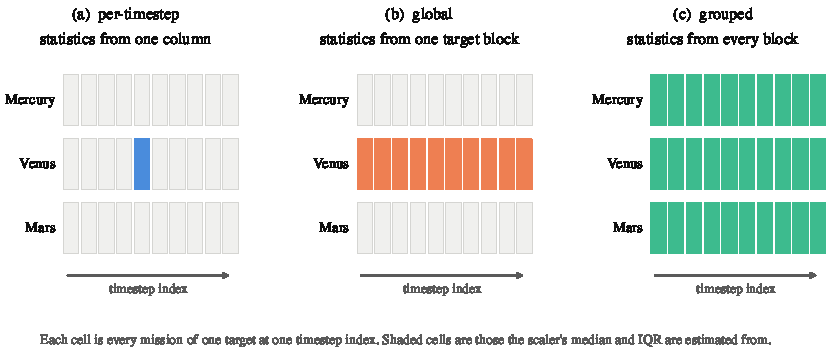
\includegraphics[width=\textwidth]{fig1_conditions.pdf}
\caption{The three normalisation settings, and the only thing that differs between them: which part of the data the scaler's median and IQR are estimated from. Everything else in the training pipeline is identical.}
\label{fig:conditions}
\end{figure*}

It is worth being explicit about why the third setting is not a straw man. Fitting one RobustScaler on a concatenated training set is what you get by following almost any standard pipeline tutorial. Nothing warns you, and the result looks like a correctly normalised array.

\section{Grouped-Normalisation Collapse}

\subsection{Why it happens}

A mission's features sweep a wide range over its flight, and different targets occupy ranges that differ by orders of magnitude. A scaler fitted over a pooled set therefore takes its scale from the largest source of variation in the pool. What the screen actually has to discriminate is neither of those things: it is the spread between missions at a given point in the flight, which is small by comparison. Pooling divides that spread by a denominator chosen for something else, squashing the useful signal toward zero while leaving the between-group structure untouched. The network is then asked to amplify a difference that has been pushed to the edge of what gradient descent can pick up, and Pre-LN layer normalisation removes much of what survives.

We measure this as the signal ratio: the mean across-mission standard deviation of the normalised features, computed inside the observed window only. The restriction matters more than it might seem. Averaged over the whole flight the metric is useless, because late timesteps carry enormous across-mission spread, because failing trajectories have physically diverged by then, and that swamps the early signal, making every condition look healthy. The model commits at 40\%, so the quantity that matters is the spread inside the prefix it actually sees.

\subsection{The controlled ablation}

\begin{table*}[!t]
\centering
\caption{Normalisation ablation. Identical architecture, seed and split; only the pooling differs. 'sig' is the mean within-timestep standard deviation of the normalised features in the observed window. 'std' is the standard deviation of P(fail) over the held-out split, the quantity that identifies a collapse, as against a model that is merely inaccurate.}
\label{tab:ablation}
\setlength{\tabcolsep}{4pt}
\footnotesize
\begin{tabular}{lrrrrrrrrr}
\toprule
 & \multicolumn{3}{c}{per-timestep} & \multicolumn{3}{c}{global} & \multicolumn{3}{c}{grouped} \\
\cmidrule(lr){2-4}\cmidrule(lr){5-7}\cmidrule(lr){8-10}
Target & sig & AUC & std & sig & AUC & std & sig & AUC & std \\
\midrule
Venus & 0.7681 & 0.9999 & 4.72e-01 & 0.0518 & 0.9947 & 4.50e-01 & 0.0023 & 0.6037 & 3.11e-05 \\
Mars & 1.0829 & 0.9994 & 4.33e-01 & 0.0472 & 0.9972 & 4.00e-01 & 0.8005 & 0.9422 & 4.06e-01 \\
Mercury & 0.7686 & 0.9994 & 4.27e-01 & 0.1321 & 0.9970 & 4.23e-01 & 0.0484 & 0.9069 & 4.25e-01 \\
Jupiter & 0.7708 & 1.0000 & 4.78e-01 & 0.0763 & 1.0000 & 4.78e-01 & 0.0247 & 0.9997 & 4.75e-01 \\
\bottomrule
\end{tabular}
\end{table*}

The decomposition is the first result. Pooling across timesteps within a single target squashes the signal by one to two orders of magnitude, and yet the network keeps working: it survives on all 4 targets, losing at most a few thousandths of AUC. Pooling across a group is a different animal. On Venus it is catastrophic --- held-out output standard deviation 3.11e-05, which is to say the network emits one number for every mission regardless of what it is shown, with AUC falling from 0.9999 to 0.6037.

\begin{figure*}[!t]
\centering
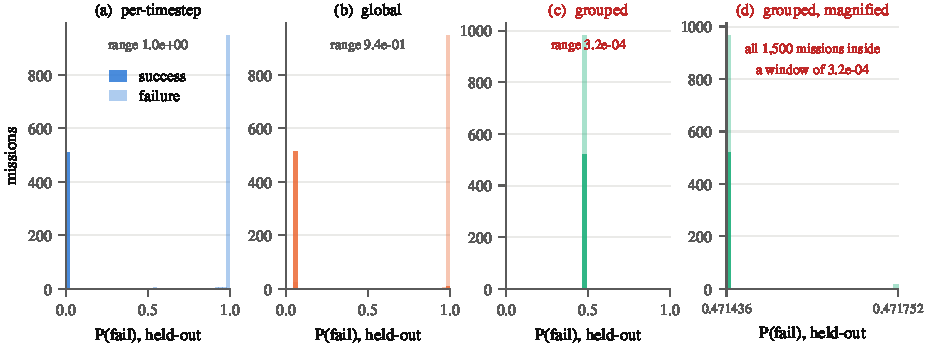
\includegraphics[width=\textwidth]{fig2_collapse.pdf}
\caption{Held-out P(fail) on Venus under each setting, split by ground truth. Under per-timestep and global normalisation the two populations sit at opposite ends of the axis. Under grouped normalisation every mission receives essentially the same number; panel (d) magnifies that spike and shows the full range of the predictions is about three ten-thousandths wide. This is what distinguishes a collapse from a bad model.}
\label{fig:collapse}
\end{figure*}

Fig.~\ref{fig:collapse} is the reason we use the word 'collapse' rather than 'underfitting'. A low AUC on its own is ambiguous: it is what you would see from a model that has learned something weak or wrong. A held-out prediction distribution three ten-thousandths wide is not ambiguous. The network has stopped being a function of its input.

The second result is that the collapse is selective, and we report this rather than only the case that breaks. On the other 3 targets the same manipulation costs between 0.0003 and 0.0925 AUC and leaves the output varying normally. Severity does not follow the signal ratio on its own either. Jupiter's signal is compressed to 0.0247, lower than Mercury's 0.0484, and yet Jupiter loses 0.0003 AUC where Mercury loses 0.0925, because Jupiter's task is separable enough that even a badly attenuated signal is sufficient. Compression is necessary for the collapse but not sufficient; how hard the underlying task is modulates it. A rule of the form 'it collapses when the ratio drops below X' is therefore not supported by these data, and we do not claim one. Fig.~\ref{fig:signal} makes the counter-example visible.

\begin{figure}[!t]
\centering
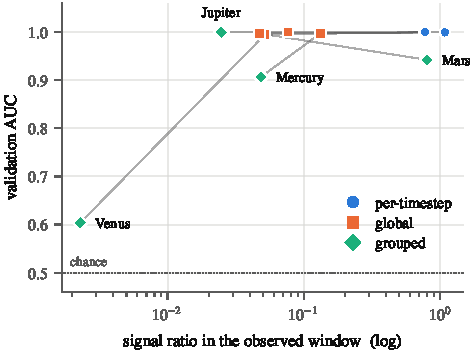
\includegraphics[width=\columnwidth]{fig3_signal_vs_auc.pdf}
\caption{Signal ratio against validation AUC. If compression alone explained the collapse these points would lie on a curve. Jupiter sits at a lower signal ratio than Mercury and loses almost nothing, so they do not.}
\label{fig:signal}
\end{figure}

One note on scope. This ablation isolates normalisation and nothing else: a separate model is trained per target, and only the statistics are pooled. The production failure that prompted the study also shared a single model across the group, which compounds the problem, since one trunk then has to serve targets whose inputs have all been flattened toward a common constant. The numbers here are therefore a lower bound on the damage the full configuration does. They establish that pooled normalisation is sufficient on its own to destroy a target, not that this is a complete reconstruction of the original incident.

\subsection{The baseline signs off on the broken configuration}

\begin{table}[!t]
\centering
\caption{XGBoost on the identical normalised window, under each setting. The tree does not react to the preprocessing that destroys the network.}
\label{tab:invariance}
\setlength{\tabcolsep}{4pt}
\footnotesize
\begin{tabular}{lrrrr}
\toprule
Target & per-timestep & global & grouped & spread \\
\midrule
Venus & 1.0000 & 1.0000 & 1.0000 & 0.0000 \\
Mars & 0.9996 & 0.9998 & 0.9998 & 0.0002 \\
Mercury & 0.9997 & 0.9998 & 0.9998 & 0.0001 \\
Jupiter & 1.0000 & 1.0000 & 1.0000 & 0.0000 \\
\bottomrule
\end{tabular}
\end{table}

Under the grouped setting the tree reports AUC 1.0000 on Venus, the target where the network has collapsed to a constant at AUC 0.6037. Across all targets the tree's AUC moves by at most 0.0002 between settings, so for practical purposes it cannot see the choice at all. Someone who runs it to check whether the features carry signal, which is the standard move and the correct instinct, gets an unambiguous yes, and reasonably concludes that the deep model needs tuning rather than that the pipeline is broken.

\begin{figure}[!t]
\centering
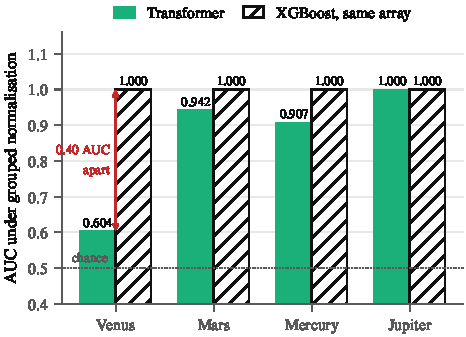
\includegraphics[width=\columnwidth]{fig4_baseline_blindness.pdf}
\caption{Both models under grouped normalisation, on the same arrays. The tree is at the ceiling on every target, including the one where the network is barely above chance.}
\label{fig:blindness}
\end{figure}

This is the methodological point, and it is worth stating carefully, because the baseline is not wrong. The information really is present, and a tree really can use it. The baseline is uninformative about the question that was actually being asked, which is whether the network can use it. Invariance to feature scaling, normally an excellent reason to reach for a tree as a diagnostic, is exactly what makes it blind here. The check and the defect are orthogonal by construction, so no amount of care in running the check would have helped.

\subsection{A diagnostic that does catch it}

Accuracy on a mixed validation set does not catch the collapse, because a per-group constant ranks the groups correctly and a pooled metric rewards that. Two checks do catch it:

\begin{itemize}
  \item Prediction spread within a group. A collapsed model produces almost no variation in its output across inputs. This is a property of the predictions alone, needs no labels, and cleanly separates collapse from ordinary underfitting, which produces predictions that are wrong but still vary.
  \item Tree against network under identical preprocessing. A large gap in the tree's favour, with both fed the same array, says the network cannot exploit information that is present, rather than that the information is absent.
\end{itemize}

Both are cheap, and neither requires you to suspect this specific defect in advance, which is the property that makes a diagnostic worth having. We would recommend reporting per-group prediction spread alongside aggregate metrics whenever a model is trained on grouped data with heterogeneous scales. In our case it would have turned a problem that survived several review cycles into a one-line check.

\section{Does It Reproduce Across Seeds?}

An obvious objection to everything above is that it describes one run. A single collapse at AUC 0.6037 could be an unlucky initialisation. We therefore repeated the full ablation across 5 seeds, each of which redraws the train/validation/test partition as well as the initialisation.

\begin{table}[!t]
\centering
\caption{Validation AUC across 5 seeds, mean $\pm$ standard deviation, and the number of seeds on which the grouped run collapsed to a constant output.}
\label{tab:multiseed}
\setlength{\tabcolsep}{4pt}
\footnotesize
\begin{tabular}{lrrr}
\toprule
Target & per-timestep AUC & grouped AUC & collapsed \\
\midrule
Venus & 0.9998 $\pm$ 0.0001 & 0.6912 $\pm$ 0.1710 & 4/5 \\
Mars & 0.9992 $\pm$ 0.0004 & 0.9457 $\pm$ 0.0104 & 0/5 \\
Mercury & 0.9997 $\pm$ 0.0002 & 0.9118 $\pm$ 0.0040 & 0/5 \\
Jupiter & 0.9999 $\pm$ 0.0002 & 0.9997 $\pm$ 0.0003 & 0/5 \\
\bottomrule
\end{tabular}
\end{table}

\begin{figure}[!t]
\centering
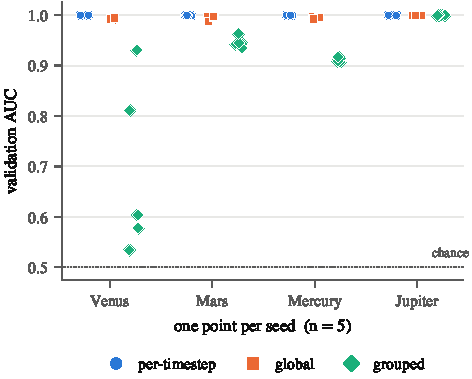
\includegraphics[width=\columnwidth]{fig7_multiseed.pdf}
\caption{Every seed plotted individually rather than summarised as an interval. With n = 5 the spread of the raw points is the honest summary.}
\label{fig:multiseed}
\end{figure}

The compression itself does not depend on the seed. Venus's signal ratio under grouped normalisation lands between 0.00222 and 0.00232 across all 5 runs, a spread of 5\% against the 335x compression itself, because it is a property of the preprocessing and the data, not of the optimiser. The healthy condition is stable too: per-timestep AUC moves by at most 0.0004 between seeds. Mars, Mercury and Jupiter never collapse under any seed. 

What does depend on the seed is whether the network escapes. Venus collapses to a constant on 4 of 5 seeds, with held-out prediction spread between 1.57e-05 and 4.84e-05, four orders of magnitude below the 4.66e-01 it reaches under correct normalisation. On the remaining seed it does not fully collapse, but it does not recover either: prediction spread 3.64e-02, still an order of magnitude short, at AUC 0.9305 against 0.9999 healthy. So the preprocessing reliably creates the conditions for the collapse, and the collapse is the usual but not the certain outcome.

This is the practical argument for the prediction-spread diagnostic recommended above. Across these runs Venus's grouped AUC spans 0.5338 to 0.9305, a range that overlaps what a merely-degraded target scores. Mercury sits inside it on every seed while discriminating normally. AUC therefore cannot tell the two states apart. Prediction spread can: the collapsed runs and every healthy run are separated by orders of magnitude with nothing in between. If you are going to watch one number for this failure, watch that one.

The baseline's blindness replicates more cleanly still. Across 5 seeds, 4 targets and three normalisation settings, 60 fitted trees in total, the tree's AUC never leaves the range 0.9989 to 1.0000, and within any one seed and target it moves by at most 0.0003 between settings. There is no seed on which the baseline notices. That matters more than the collapse count: the collapse is one target's misfortune, but a check that cannot fail is a property of the check.

\section{Failing to Reach a Signal That Is Present}

\label{sec:rare}

A second failure shows up even when the normalisation is correct. On Uranus, the failure mode 'surface\_impact' accounts for 91 of 4,639 training failures. A tree fitted to the same normalised 40-step window separates that mode from success at AUC 1.0000, with recall 1.0000. The sequence model's recall on it is 0.0000 at its operating point.

\begin{table}[!t]
\centering
\caption{Rare-mode oversampling sweep on Uranus. Increasing the sampling weight on the rare mode does not recover it, and does not disturb anything else either.}
\label{tab:rare}
\setlength{\tabcolsep}{4pt}
\footnotesize
\begin{tabular}{lrrrr}
\toprule
alpha & resample & test F1 & all-mode recall & rare-mode recall \\
\midrule
0.00 & 1.0x & 0.9938 & 0.9877 & 0.0000 \\
0.50 & 5.1x & 0.9938 & 0.9877 & 0.0000 \\
1.00 & 19.2x & 0.9938 & 0.9877 & 0.0000 \\
\bottomrule
\end{tabular}
\end{table}

\begin{figure}[!t]
\centering
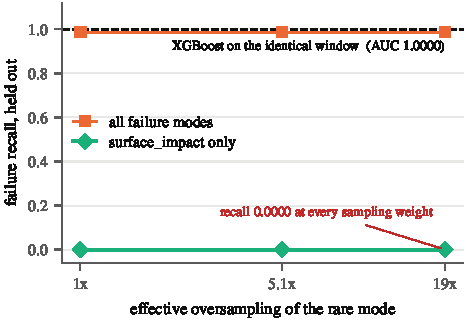
\includegraphics[width=\columnwidth]{fig5_rare_mode.pdf}
\caption{Recall against oversampling weight. The horizontal line is a tree on the identical window. The rare-mode curve does not move.}
\label{fig:rare}
\end{figure}

Because both models consume the same array and one of them separates the classes cleanly, the information is present and the sequence model's failure is an optimisation limit rather than an information limit. Resampling does not close the gap, which rules out the simplest explanation. We are careful not to overclaim the cause: whether it is the loss landscape, the CLS pooling discarding a cue that is localised in time, or the binary head being dominated by the majority mode, we do not know. Probing the trunk representation for linear separability of the rare mode would narrow it down, and that is the next experiment rather than a result we have.

Two denominators are worth stating, because this number is easy to quote misleadingly. Relative to the majority failure mode the rare mode is oversampled by roughly 45x at the strongest setting. Relative to uniform sampling over the training set, which is what the sampler actually applies, the factor is 19.23x. We report the latter, because it describes what the optimiser saw.

The sweep was repeated across 5 seeds, each of which redraws the split and therefore the rare mode itself. The gap replicates and the extremes do not: sequence recall on the rare mode ranges 0.0000 to 0.1429 across every seed and sampling weight, against a tree on the identical window at recall 0.9333 to 1.0000 and AUC 0.9997 to 1.0000. On every seed the sampling weight makes no difference whatsoever: recall is identical at all three settings within a seed, so the flat line in the figure is not a property of one run.

\section{Where the Screen Actually Belongs}

\label{sec:econ}

\begin{table*}[!t]
\centering
\caption{Screening economics. Compute is charged in propagation-days, which span a \textasciitilde{}100x range across the seven targets. Thresholds are fitted on validation and reported on the untouched test split, so the recall column is measured out of sample rather than achieved by construction.}
\label{tab:econ}
\setlength{\tabcolsep}{4pt}
\footnotesize
\begin{tabular}{lrrr}
\toprule
Screen & Compute saved & Good missions lost & Failure recall \\
\midrule
\textbf{T0: six launch parameters, before propagating} & \textbf{64.5\%} & \textbf{0.76\%} & \textbf{99.06\%} \\
T40: telemetry Transformer at 40\% & 38.3\% & 0.21\% & 98.87\% \\
Cascade: T0 where confident, else T40 & 65.0\% & 1.62\% & 99.94\% \\
\bottomrule
\end{tabular}
\end{table*}

\begin{figure*}[!t]
\centering
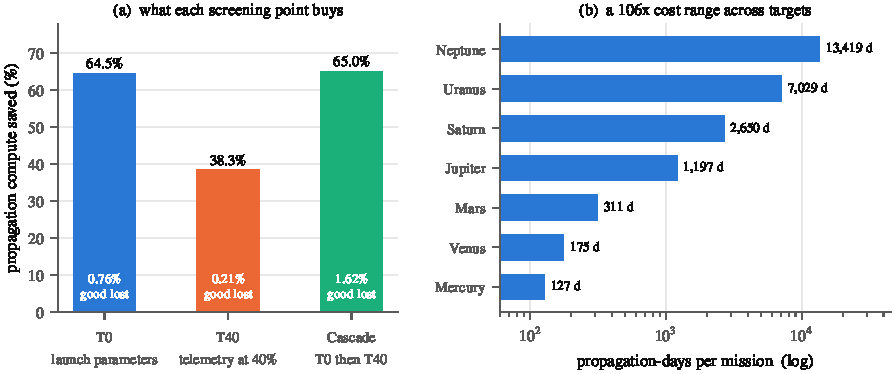
\includegraphics[width=\textwidth]{fig6_economics.pdf}
\caption{(a) What each screening point buys and what it costs. (b) Why the weighting is not uniform: per-mission propagation cost spans two orders of magnitude, so the value of a screen is dominated by the outer targets.}
\label{fig:econ}
\end{figure*}

Having gone to the trouble of fixing the sequence model, the honest conclusion is that it should not be used. A six-feature classifier over the injection parameters, evaluated before any propagation happens at all, saves 64.5\% of compute against the telemetry model's 38.3\%, at a comparable cost in good missions destroyed. Accuracy is also flat from 10\% to 40\% observed. The reason is structural rather than a modelling failure: the simulator is deterministic, so the outcome is a fixed function of the injection offsets and the trajectory is their integral. It cannot carry information the parameters do not already have.

This is not an argument that the task is trivial. Logistic regression on the same six features scores between 0.4824 and 0.5410 AUC (chance) on every target, so the map from parameters to outcome is strongly nonlinear and does need a learned model. It just does not need a temporal one. A sequential screen earns its place only where the outcome is not settled at injection: mid-flight stochasticity, unmodelled dynamics, sensor noise, or campaigns where the launch parameters were never recorded. Reinforcement-learning trajectory work that certifies policies through dispersed Monte Carlo campaigns \cite{zavoli2021rl} is a natural setting for exactly that.

We include this section because it bounds the practical significance of everything before it. The methodological findings apply to any grouped sequence-modelling pipeline; the application that produced them turns out not to need a sequence model. A reviewer who discovers that on their own is in a worse position than one who is told.

One methodological note on this table, since it cuts against the conclusion we draw. An earlier version was produced under two selection biases: thresholds were fitted on the test labels, and the evaluation set overlapped the sequence model's validation split. Both flattered T40, the screen this section argues against. Removing them moved the headline by less than 0.1 percentage points, so the negative result survives its own correction, which is the strongest form the claim can take.

\section{Limitations}

\begin{itemize}
  \item Seeds. Results are replicated across 5 seeds, which is enough to rule out an unlucky initialisation but not enough to support a tight confidence interval. We report the spread of the individual runs rather than a fitted interval. The collapse itself occurs on 4 of 5; we do not have the sample size to say what governs the exception.
  \item One domain. The collapse is shown on one corpus. We describe the mechanism in terms of a variance ratio that is not specific to astrodynamics, but we have not reproduced it on a second dataset, and until we do, any predictive threshold on that ratio is a conjecture rather than a finding.
  \item Four targets in the ablation. The collapse is observed on one target out of four. The baseline-blindness result, which is the methodological half, holds on all four.
  \item Synthetic and deterministic. No execution error, no unmodelled accelerations, no sensor noise, and every mission of a target shares a time base. That shared time base is what makes per-timestep standardisation work at all, and it is a property of the generator rather than of real campaigns.
  \item No real mission data. This is the largest external-validity gap. Public benchmarks of real satellite telemetry now exist \cite{kotowski2024esaadb,hundman2018detecting} and are the obvious next target for the diagnostic.
\end{itemize}

\section{Conclusion}

Sharing a feature scaler across groups whose scales differ can reduce a deep model to a per-group constant, while a tree on the identical arrays reports the task as solved. None of the pieces are exotic. The preprocessing choice is one that a standard pipeline makes by default. The model is a plain Transformer. The baseline is the one most people would reach for. And the standard defence (check a simple baseline) is invariant to the defect by construction, so it cannot fail the broken model.

The fix, per-group normalisation, is not novel and we do not claim it is. The contribution is the detection problem: that a routine check certifies a broken configuration, and that a different check, costing essentially nothing, catches it. Reporting the spread of predictions within a group alongside aggregate metrics would have caught ours immediately.

\section{Code and Data Availability}

Everything in this paper (the experiment scripts, the JSON artifacts every number is read from, the figure code, and the source of this document) is at \url{https://github.com/Haise-727/gmat-pred}. A short map of where things are:

\begin{itemize}
  \item src/ml/ holds the experiments. norm\_ablation.py produces Table I, baseline\_invariance.py Table II, rare\_mode\_sweep.py Table IV, prune\_economics.py Table V. splits.py is the single definition of the train/validation/test partition that all of them share.
  \item src/ml/model.py is the Transformer, and planet\_config.py the target list, cadences and the recorded reason the Moon is excluded.
  \item reports/ holds the measured artifacts. Every table and figure here is read from one of these JSON files; multiseed\_paper/ holds the per-seed runs behind Table III.
  \item docs/paper/ builds this document. content.py holds the prose and makes the tables from the artifacts; figures.py draws every figure from the same artifacts; render\_latex.py and build\_paper.py render the LaTeX and Word versions. No number in the paper is typed in by hand.
  \item docs/RESEARCH\_LEDGER.md is the full decision history, including two analyses that were invalidated by a positional join and the corrections that replaced them. docs/LIMITATIONS.md states what the results do not support.
\end{itemize}

The per-target .npz extracts the experiments read (roughly 70 MB each) are derived from a 71 GB mission table that is too large to host in the repository. The scripts below regenerate the artifacts from those extracts; ORBITGUARD\_DATA points at the full table for the economics analysis, which is the only experiment that needs it.

\begin{lstlisting}
export ORBITGUARD_DATA=/path/to/dataset

# Primary results, seed 42
python -m src.ml.norm_ablation          # Table I
python -m src.ml.baseline_invariance    # Table II
python -m src.ml.rare_mode_sweep        # Table IV
python -m src.ml.prune_economics        # Table V

# Replication, one pass per seed (Table III, Section V)
for S in 0 1 2 3; do
  python -m src.ml.norm_ablation --seed $S \
      --out reports/multiseed_paper/normalisation_ablation_seed$S.json
  python -m src.ml.baseline_invariance --seed $S \
      --out reports/multiseed_paper/baseline_invariance_seed$S.json
  python -m src.ml.rare_mode_sweep --seed $S \
      --out reports/multiseed_paper/rare_mode_sweep_seed$S.json
done

# The document
python docs/paper/collect_traces.py     # Fig. 2 data
python docs/paper/figures.py            # all figures
python docs/paper/render_latex.py       # this document
\end{lstlisting}

\bibliographystyle{IEEEtran}

\bibliography{references}

\end{document}
